% Please give the surname of the lead author for the running footer
\leadauthor{Tosheva \& Laine}

% info about NM-BC format: https://www.nature.com/nmeth/about/content

\title{NanoJ: a high-performance open-source super-resolution microscopy toolbox}
%NM-BC: The title is limited to 10 words (or 90 characters)
\shorttitle{NanoJ}

% Use letters for affiliations, numbers to show equal authorship (if applicable) and to indicate the corresponding author
\author[1,2\space *]{Kalina L. Tosheva}
\author[1-3\space *]{Romain F. Laine}
\author[1,2,4]{Nils Gustafsson}
\author[1,2,4]{Robert D. M. Gray}
\author[1,2]{Pedro Almada}
\author[1]{David Albrecht}
\author[1,6]{Gabriel Tarrason Risa}
\author[7]{Ann-Christin Lindås}
\author[1,6]{Buzz Baum}
\author[1]{Jason Mercer}
\author[5]{Christophe Leterrier}
\author[1-3\space\Letter]{Pedro M. Pereira}
\author[1-3\space\Letter]{Si\^{a}n Culley}
\author[1-3\space\Letter]{Ricardo Henriques}

\affil[1]{MRC-Laboratory for Molecular Cell Biology. University College London, London, UK}
\affil[2]{Department of Cell and Developmental Biology, University College London, London, UK}
\affil[3]{The Francis Crick Institute, London, UK}
\affil[4]{Centre for Mathematics and Physics in Life Sciences and Experimental Biology (CoMPLEX), University College London, London, UK}
\affil[5]{Aix Marseille Université, CNRS, INP UMR7051, Marseille, France}
\affil[6]{Institute for the Physics of Living Systems, University College London, London, UK}
\affil[7]{Department of Molecular Biosciences, The Wenner-Gren Institute, Stockholm University, Stockholm, Sweden}

\affil[*]{These authors contributed equally.}

\maketitle

%TC:break Abstract
\begin{abstract}
%Lets try to keep the abstract between 70-150 words, I have noticed no guidance

Super-Resolution Microscopy has become essential for the study of many nanoscale biological processes. This type of imaging considerably relies on specialised image analysis tools to routinely process large volumes of recorded data and robustly extract underlying quantitative information. In recent years, our team has built an image analysis framework for Super-Resolution Microscopy that is high-performance, open-source and ease of use. We name it NanoJ - a reference to the popular ImageJ software it was developed for. In this paper, we highlight the current capabilities of NanoJ for use in several essential steps of microscopy studies: spatiotemporal alignment of raw data (NanoJ-Core), Super-Resolution image reconstruction (NanoJ-SRRF), image quality assessment (NanoJ-SQUIRREL), structural modelling (NanoJ-VirusMapper) and control of the sample environment (NanoJ-Fluidics). We are constantly expanding NanoJ with the aim to improve quantitative analysis and reliability of biological microscopy studies.

\end {abstract}
%TC:break main
%the command above serves to have a word count for the abstract

\begin{keywords}
    ImageJ | Fiji | Super-Resolution Microscopy | Image Analysis | Fluidics | Resolution | Quantitative imaging | Modelling
\end{keywords}

\begin{corrauthor}
    p.pereira\at ucl.ac.uk, s.culley\at ucl.ac.uk, r.henriques\at ucl.ac.uk
\end{corrauthor}

%%%%%%%%%%%%%%%%
% Introduction %
%%%%%%%%%%%%%%%%
% ------------------------------------------------------------------------------------------------------------------------------------

\subsection*{Introduction}
Fluorescence microscopy has been ubiquitously used in biological studies since its invention in the 20\textsuperscript{th} century. It underpins most research observing structures and interactions between specifically labelled molecules, and allows the quantification of their dynamic behaviour in living cells \cite{rino2009frontiers}. However, extracting biologically relevant quantitative information from fluorescence microscopy data requires specialised digital processing and analysis \cite{wheeler2017standard}. In recent years, Super-Resolution Microscopy (SRM) techniques \cite{betzig2006imaging,rust2006sub,hell1994breaking} have extended the spatial resolving power of fluorescence microscopy beyond that of the diffraction limit. Most SRM techniques generate large quantities of data, often reaching several gigabytes of raw data for a single image, and thus require high-performance image analysis tools.  Several SRM image processing packages are available, such as ThunderSTORM \cite{ovesny2014thunderstorm}, LAMA \cite{Malkusch2016LAMA} and SIMcheck \cite{schermelleh2015simcheck}, but each of these is focused on a specific type of SRM modality.
  
 %TC:ignore
 \begin{figure}[!t]
    \centering
    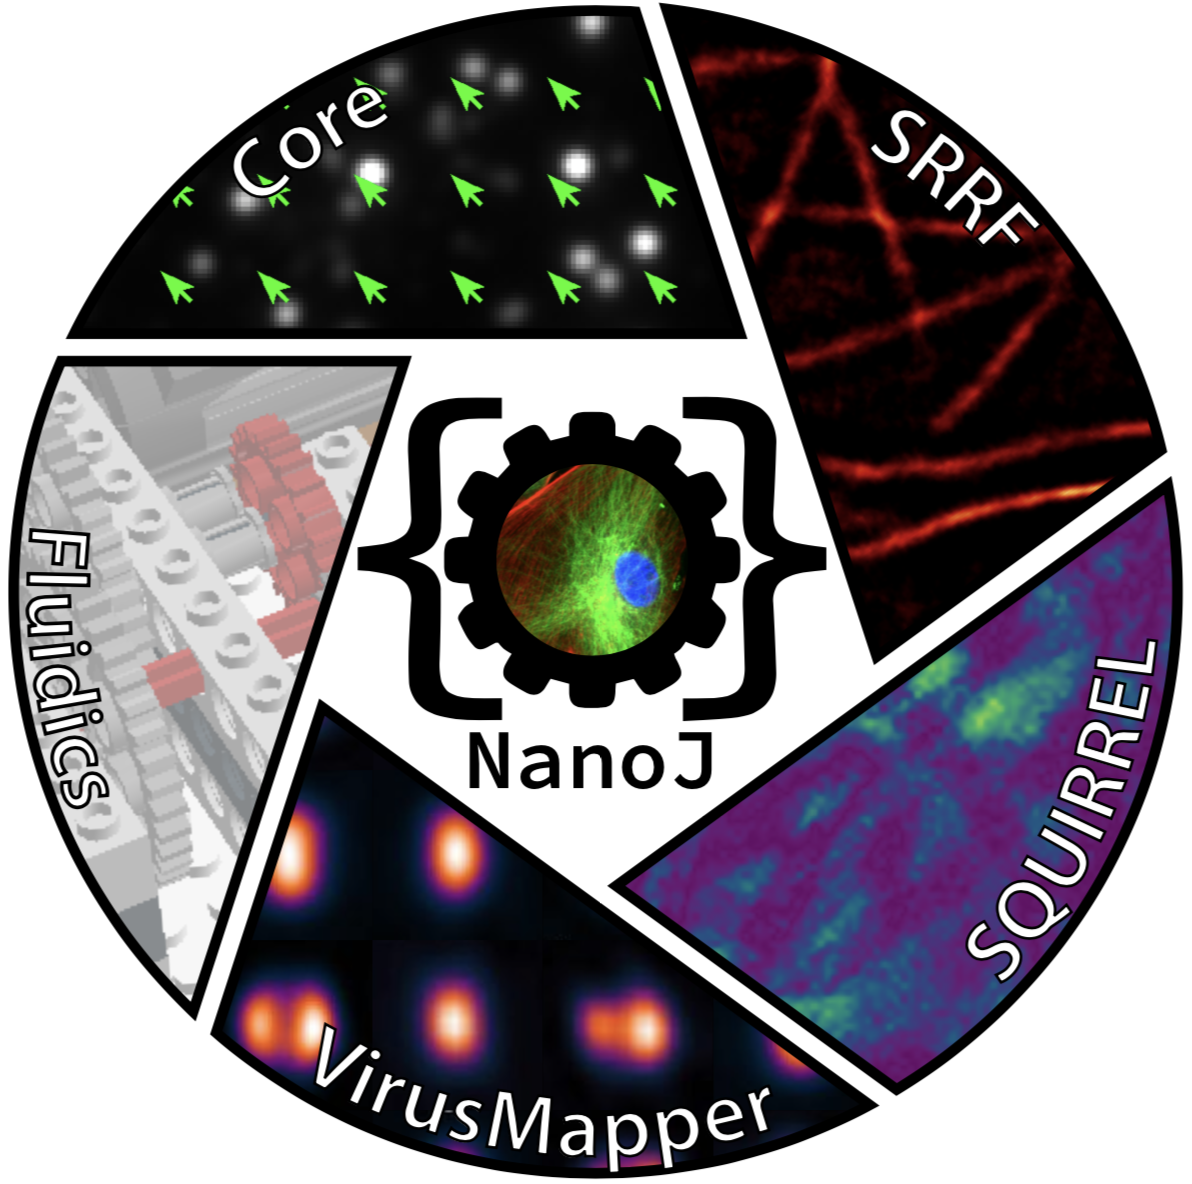
\includegraphics[width=\linewidth]{Figures/FigureMain_v3.png}
    \caption{\textbf{NanoJ framework.} Currently NanoJ consists of 5 modules dedicated to enable super-resolution imaging and analysis.}
    \label{fig:GeneralDiagram}
 \end{figure}
 %TC:endignore
 
%  linewidth: \printinunitsof{in}\prntlen{\linewidth}

 Here, we present NanoJ, a highly versatile set of image acquisition and analysis methods developed to improve microscopy experiments, with a particular focus on the demands of live-cell SRM. NanoJ is available as a series of ImageJ-based plugins which can be used independently or concomitantly to obtain high-fidelity images from which qualitative and quantitative information can be extracted. NanoJ is comprised of (Fig. \ref{fig:GeneralDiagram}): \textbf{NanoJ-Core} - a set of general image correction tools which include drift correction and channel realignment, both based on cross-correlation analysis; \textbf{NanoJ-SRRF} - an analytical approach capable of extracting super-resolution data from a short burst sequence of diffraction-limited images, which can be acquired using most microscopes \cite{gustafsson2016fast,culley2018srrf}; \textbf{NanoJ-SQUIRREL} - an algorithm to evaluate resolution and the presence of artefacts in super-resolution images \cite{culley2018quantitative}; \textbf{NanoJ-VirusMapper} - a single-particle analysis method to generate nanoscale models of repetitive meta-stable biological structures such as viruses \cite{Gray2016,Gray2017,gray2018nanoscale}; \textbf{NanoJ-Fluidics} - a software interface to control fluidic hardware devices, enabling automation, e.g. of multiplexed experiments \cite{almada2018automating}. While these methods were originally developed to address specific biological questions, NanoJ is aimed at solving common imaging problems with broad applications. Thus the NanoJ framework is compatible with a multitude of fluorescence microscope setups and experimental protocols. 
 
\subsection*{The NanoJ framework}
 NanoJ has been designed to integrate with the popular ImageJ or Fiji image analysis software \cite{abramoff2004image,schindelin2012fiji}, being easily installed as a standard set of plugins. NanoJ is fully open-source and user-friendly, making use of state-of-the-art algorithms and code execution strategies. The graphical user interfaces (GUIs) are straightforward to use and its routines can be easily integrated within larger image analysis pipelines through the ImageJ macro language.

 NanoJ is composed by individual modules with corresponding manuals. It is designed to be an accessible tool for both non-expert users and developers. NanoJ is implemented in both Java (\href{https://www.java.com/}{https://www.java.com/}) and OpenCL (\href{https://www.khronos.org/opencl}{https://www.khronos.org/opencl}), the latter language being used for high-performance analysis of image data through the use of Graphical Processing Units (GPUs). As of date, it encompasses four Java ARchive (JAR) packages - NanoJ-SRRF, NanoJ-SQUIRREL, NanoJ-VirusMapper, NanoJ-Fluidics - that all depend on a central package - NanoJ-Core. The core package hosts the libraries that enable high-performance GPU-based computing analysis and a set of basic image analysis helper methods. The modular nature of NanoJ means that its components can be updated independently and the framework can be easily extended by appending new analytic packages.

\subsection*{NanoJ-Core: Drift Correction}
Sample drift commonly occurs during the acquisition of SRM data, often as a result of gradual changes in the temperature of system components. Drift introduces motion blur artefacts and thereby a loss of resolution. While most modern microscopes have an active focus-lock device that stabilises the motion of the sample in the axial direction (minimizing focal drift), the sample will still be prone to lateral movement (Fig. \ref{fig:DriftCorrection}a). However, in the case where the raw data is made up of a sequence of consecutive frames acquired rapidly, as is common in SRM methods such as Single Molecule Localization Microscopy (SMLM) \cite{betzig2006imaging,rust2006sub} or fluctuation-based approaches \cite{gustafsson2016fast,dertinger2009fast,cox2012bayesian}, this lateral drift can be estimated (Fig. \ref{fig:DriftCorrection}b) and analytically corrected via post-processing (Fig. \ref{fig:DriftCorrection}c-d).
 
  %TC:ignore
 \begin{figure}[!t]
    \centering
    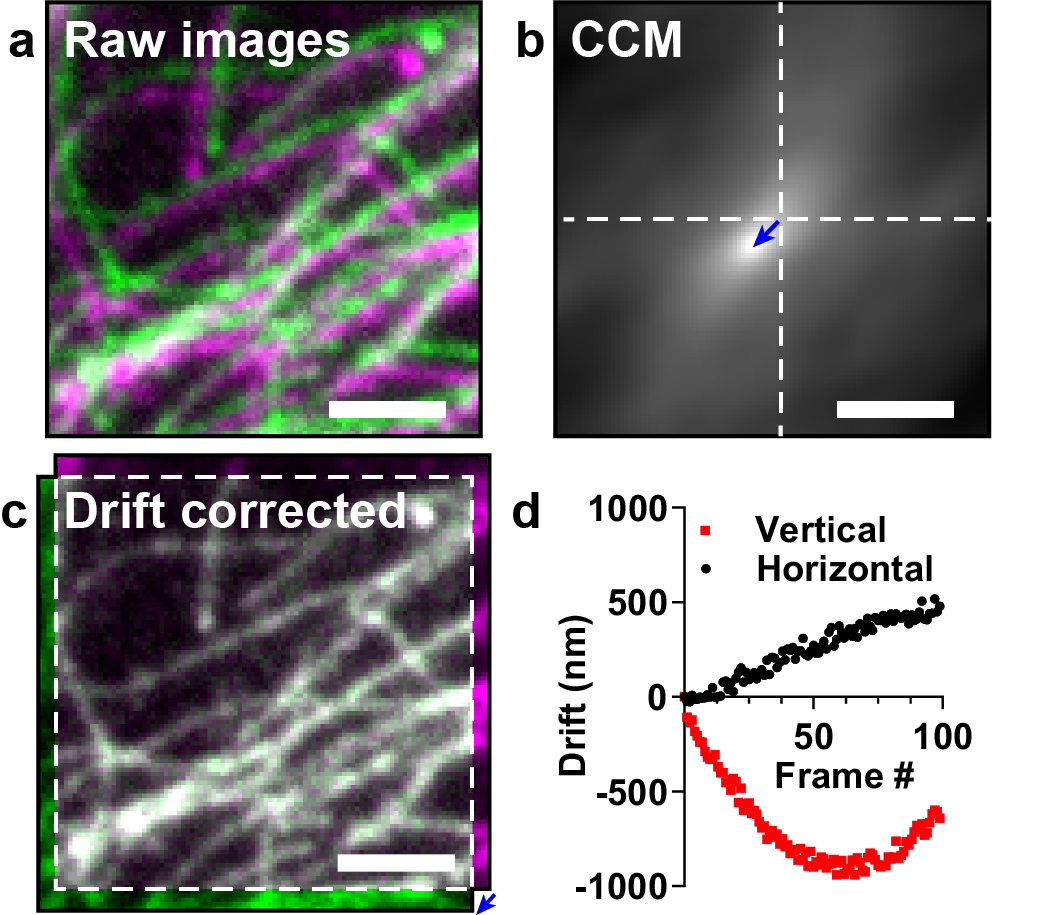
\includegraphics[width=\linewidth]{Figures/FigureDrift_v2.png}
    \caption{\textbf{Drift correction with NanoJ-Core.} \textbf{a)} Composite image of two frames of the same field-of-view with visible drift. \textbf{b)} Cross-correlation map between the two frames shown in a). The vector position of the maximum indicates the linear shift between the two frames. \textbf{c)} Overlay of the two frames after drift correction using NanoJ-Core. \textbf{d)} Example vertical and horizontal drift curves obtained from 100 consecutive frames.}
    \label{fig:DriftCorrection}
 \end{figure}
 %TC:endignore

 NanoJ breaks the task of drift correction into two distinct parts: estimation, followed by translation. As a first step NanoJ-Core estimates the linear drift between two images by calculating their cross-correlation matrix (CCM) (see Fig.\ref{fig:DriftCorrection}b). The location of the peak intensity in the CCM determines the linear shift between the two images and is precisely estimated by up-scaling the CCM, using a bicubic-spline interpolation, thus achieving sub-pixel accuracy. Depending on the type of acquisition, the reference frame can either be the first frame of the raw data (e.g. for a fixed sample) or the preceding SRM frame (for a live sample). Fig. \ref{fig:DriftCorrection}d shows how the drift with respect to the first frames can be followed in time in a example 100 frames dataset. Once drift is estimated, the dataset can be directly corrected by analytically translating each individual frame using a bicubic-spline interpolation (Fig. \ref{fig:DriftCorrection}c). The interpolation process will change the noise properties of the resulting dataset \cite{blaysat2016effect}.
 
 For the specific case of SMLM datasets with sparse blinking, there will only be a weak correlation across frames, as there is little observable structure conserved between consecutive time points. One common strategy to alleviate this low correlation is to add fiduciary landmarks to the sample, such as static fluorescent beads. Alternatively, NanoJ-Core can temporally bin the dataset thus increasing the correlation between binned frames and allowing their shift to be more precisely estimated \cite{mlodzianoski2011sample}. 

 Drift estimation in NanoJ differs from strategies applied by other SRM algorithms, such as ThunderSTORM \cite{ovesny2014thunderstorm}, by analysing acquired unprocessed data, instead of post-processed Super-Resolution reconstructions. This allows the estimation to be decoupled from the Super-Resolution analysis strategy used, thus enabling further methods such as SRRF or SOFI \cite{dertinger2009fast} to benefit from it. Alternatively, algorithms such as NanoJ-SRRF can import the created drift-table, directly using this information during analysis without the need to pre-translate each frame in the raw dataset.

\subsection*{NanoJ-Core: Channel Alignment}

 Images captured with a fluorescence microscope in different spectral channels often appear misaligned, as a result of chromatic aberrations in the optical systems and from using different spectral filters between channels. While in conventional microscopy both of these effects can often be ignored, provided they occur at a scale smaller than the diffraction limit, their effect become non-negligible in the context of SRM \cite{erdelyi2013correcting}. Correction becomes essential when dealing with spectral misalignment in multi-colour SRM studies quantifying colocalisation or interactions between different structures \cite{bock2007two,van2009multicolor,niekamp2017high}. 
 
 The shift between different spectral channels often varies non-linearly with the position across the image, which prevents using typical CCM-based approaches, such as the one used by NanoJ-Core Drift Correction. A common approach to estimate the shift is to image a sample showing the same structure across all the relevant wavelength channels, where this structure occupies a large portion of the imaged field-of-view, e.g. a coverslip with a high-density distribution of multi-spectral beads randomly placed. This dataset can be used to extract a non-linear spatial transform for each spectral channel with respect to a reference channel (Fig. \ref{fig:ChannelAlignment}a), and these transforms can then be used to re-align all further multi-spectral dataset (Fig. \ref{fig:ChannelAlignment}b) \cite{arganda2006consistent,annibale2012identification}. 
 As a first step, NanoJ breaks the image down into small areas (here referred as blocks), which are in turn compared to the equivalent block in the reference channel (see Fig.\ref{fig:ChannelAlignment}a). Locally, the block shift can be assumed to be linear and estimated by finding the cross-correlation peak position as shown in Fig.\ref{fig:DriftCorrection}a-b. An inverse distance weighting interpolation \cite{shepard1968two} is used to smoothly determine shift values across the whole field-of-view, including the blocks that do not contain any structure in the calibration dataset. This approach allows us to extract a shift map (in both vertical and horizontal directions) that can be applied to further datasets (see Fig.\ref{fig:ChannelAlignment}b). The amplitudes of the horizontal and vertical shift maps represent the physical shift associated with each direction that needs to be locally re-aligned in the corresponding channel to the reference channel. These shift maps highlight the chromatic distortion across the field-of-view. 
 
 \begin{figure}[!t]
    \centering
    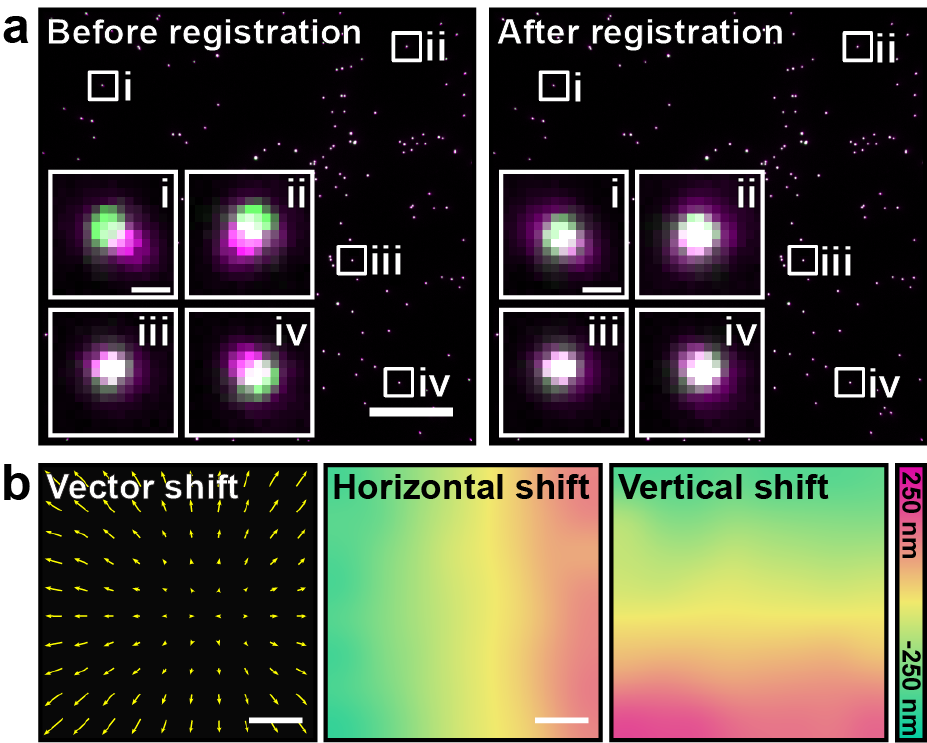
\includegraphics[width=\linewidth]{Figures/FigureChannelAlignment_v4.png}
    \caption{\textbf{Multi-colour channel alignment with NanoJ-Core.} \textbf{a)} Composite image of multi-colour TetraSpeck beads imaged in two different channels (GFP channel indicated in green and mCherry channel in magenta), prior to (left) and after (right) channel re-alignment using NanoJ-Core, acquired on a Nikon Ti2 frame with the CFI Apochromat TIRF 100XC Oil objective. Insets - individual beads from indicated locations, 1.63 x 1.63 \micro m. Scale bars: 25 \micro m. \textbf{b)} Horizontal and vertical shift maps obtaiend and applied to the data shown in a). Scale bars: 25 \micro m.}
    \label{fig:ChannelAlignment}
\end{figure}
 
 The channel alignment correction is then achieved on any multi-color dataset by creating a new image representing each channel, where the intensity value for each pixel coordinate corresponds to the intensity value from the original image at the equivalent coordinate corrected for local shift. For the cases where these coordinates are not discrete (sub-pixel shift), a bicubic-spline interpolation is used to recover pixel values in continuous space. Because the shift map can be extrapolated to continuous space, the alignment procedure obtained from diffraction-limited images can also easily be used to correct SRM datasets of any resolution. 
 
\subsection*{NanoJ-SRRF: Live-Cell Super-Resolution Imaging}

 As part of the NanoJ framework, we include our recently developed SRM reconstruction algorithm Super-Resolution Radial Fluctuations (SRRF), able to extract sub-diffraction information from a short burst of images acquired at high-speed with modern fluorescence microscopes \cite{gustafsson2016fast,culley2018srrf}. SRRF is a purely analytical approach. It alleviates the need to use toxic photoswitching-inducing buffers \cite{henriques2011palm}, specialised fluorophores \cite{dempsey2011evaluation,henriques2009palm}, damaging high-intensity illumination \cite{waldchen2015light} or specialised equipment \cite{gustafsson2000surpassing,hell1994breaking} when compared to other SRM methods \cite{betzig2006imaging,rust2006sub,gustafsson2000surpassing,hell1994breaking}.
 
 %TC:ignore
 \begin{figure}[!b]
    \centering
    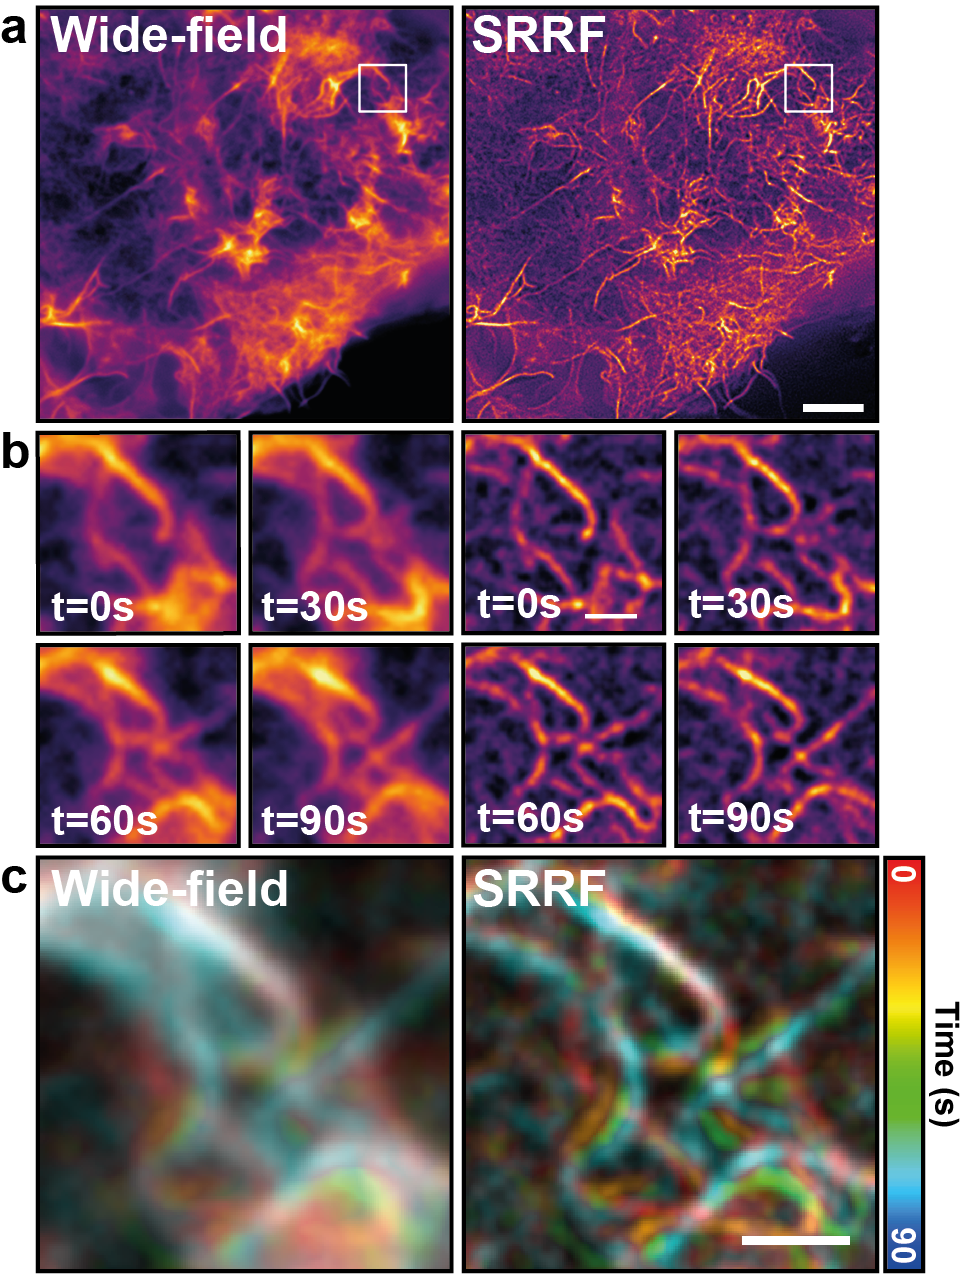
\includegraphics{Figures/FigureSRRF_v4.png}
    \caption{\textbf{Live-cell super-resolution with NanoJ-SRRF.} \textbf{a)} Comparison of wide-field (left) and SRRF reconstruction (right) obtained from a Cos7 cell expressing UtrCH-GFP. Scale bar: 5 \micro m. \textbf{b)} Time-course of the inset shown in a), obtained from  a continuous imaging at 30 ms exposure (33.3 Hz) and displayed every 30 s. Scale bar: 1 \micro m. \textbf{c)} Colour-coded time course dataset from b). Scale bar: 1 \micro m.}
    \label{fig:SRRF}
 \end{figure}
 %TC:endignore
 
 SRRF is based on similar principles to SMLM, however it does not rely on the detection of spatio-temporally isolated fluorophores. In comparison, SRRF generates a magnified pixel grid where each pixel value relates to the probability of fluorophores existing in that corresponding region of space. To do so, SRRF calculates the local radial symmetry in each sub-pixel of the magnified image using local intensity gradient information. The obtained radiality transform will be high when a point-spread-function (PSF) profile transiently becomes dominant, highlighting the presence of a fluorescent molecules in that location. Also, the fluctuation of local radiality follows the underlying natural intensity fluctuation of fluorophores, which has a distinct temporal signature to that of noise \cite{dertinger2009fast}. A temporal correlation of radial symmetries at each pixel can then be projected into a final image, where the structures of interest can be better resolved (see Fig.\ref{fig:SRRF}).

 SRRF is highly compatible with live-cell SRM and allows long time-course acquisition \cite{culley2018srrf}. Fig.\ref{fig:SRRF}a-c show a typical live-cell SRRF acquisition of a Cos7 cell expressing UtrCH-GFP (actin marker) imaged at 33.3 Hz for > 30 min with no perceivable phototoxicity. Here, SRRF allows observation of actin dynamics at super-resolution.
 
 NanoJ-SRRF, the software implementation of the SRRF algorithm, uses whenever possible GPU high-performance computing to accelerate the radial symmetry estimation. This is achieved by implementing a large set of the needed calculations in OpenCL, with a fallback of execution to CPU when a compatible graphics card is not found. NanoJ-SRRF can use a drift-table as an additional input, dynamically using its values to compensate for unwanted sample drift during the calculation of radial symmetries and temporal correlations.

\subsection*{NanoJ-SQUIRREL: Estimating Image Quality}
 In order to achieve higher resolution, all SRM techniques suffer from an additional complexity compared to conventional diffraction-limited microscopy. This complexity arises from the sample preparation requirements (SMLM), the microscope hardware (STED, SIM) and the post-acquisition image processing (SMLM, SIM). Inappropriate choices of the acquisition and reconstruction parameters can introduce artefacts within the final image and harbour the risk for false conclusions to be drawn. NanoJ-SQUIRREL (Super-resolution Quantitative Image Rating and Reporting of Error Locations) is an algorithm that highlights the presence of artefacts in super-resolution images. It does so by calculating quantitative maps showing both local SRM image quality and resolution \cite{culley2018quantitative}. These values can then be used to optimise acquisition pipelines \cite{culley2018srrf}.

 The central concept of SQUIRREL is that a diffraction-limited image and the corresponding super-resolution rendering of the same region should relate to the same underlying structure, just at different resolutions (Fig. \ref{fig:SQUIRREL}a). This concept implies that it is possible to simply blur the SRM image to decrease its resolution to achieve an equivalent diffraction-limited image. Any discrepancy between true diffraction limited and the blurred SRM will originate from artefacts or non-linearity in the reconstruction and imaging.

 NanoJ-SQUIRREL analytically formalises this notion by estimating the blurring function to apply to the SRM image and computing an error map, representing the difference between the true diffraction-limited and the blurred SRM image (Fig. \ref{fig:SQUIRREL}b). Two global quality metrics are also generated: the RSP (Resolution Scaled Pearson’s Correlation Coefficient) and the RSE (Resolution Scaled Error). The RSP can take a value in the interval [-1,1] and describes the structural agreement between the super-resolution and reference images. Here, higher values indicate better agreement, with an RSP of 1 indicating a perfect structural match. The RSE describes the sum intensity mismatch between the super-resolution and reference images; in this case lower values represent better agreement with a value of 0 indicating a perfect intensity match. Fig.\ref{fig:SQUIRREL}a and b shows super-resolution image, its corresponding diffraction-limited (widefield) image and the error map obtained from NanoJ-SQUIRREL. The three insets shown in Fig.\ref{fig:SQUIRREL}b indicate areas where typical SMLM artefact are present to different extent (mislocalization, bridging artefacts or missing localisation \cite{waldchen2015light}). 

 %TC:ignore
 \begin{figure}[!t]
    \centering
    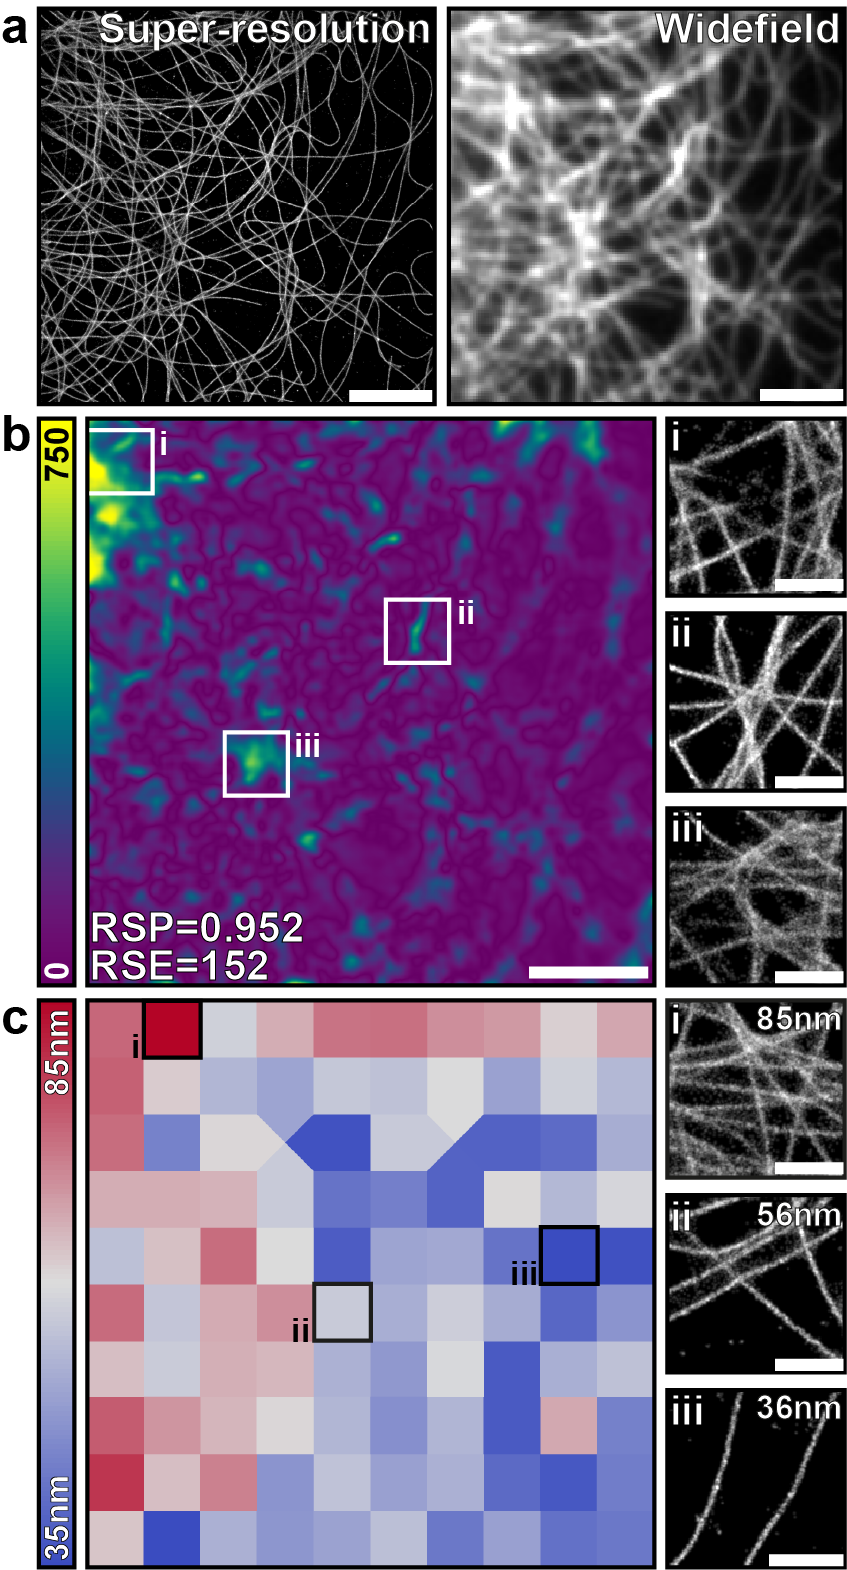
\includegraphics{Figures/FigureSQUIRREL_v1.png}
    \caption{\textbf{Quality assessment and resolution mapping with NanoJ-SQUIRREL.} \textbf{a)} A super-resolution rendering (left) and acquired widefield image (right) of fixed microtubules labelled with Alexa Fluor-647. \textbf{b)} Left: SQUIRREL error map highlighting discrepancies between the super-resolution and diffraction-limited images in (a). Right: Magnified insets of super-resolution rendering at indicated positions on error map. \textbf{c)} Left: SQUIRREL resolution map of the super-resolution image in (a). Right: Magnified insets of super-resolution rendering for indicated resolution blocks. Whole image scale bars = 5\micro m, inset scale bars = 1\micro m}
    \label{fig:SQUIRREL}
 \end{figure}
 %TC:endignore

\subsection*{NanoJ-SQUIRREL: Estimating Image Resolution}
 The purpose of SRM is to resolve finer structural detail than is achievable with conventional diffraction-limited microscopy. It is therefore useful to have an objective measurement of spatial resolution within a super-resolution image, for example to enable comparisons with known structure sizes from electron microscopy. The current standard for estimating image resolution in SRM images is Fourier Ring Correlation (FRC) \cite{nieuwenhuizen2013measuring}. This method involves comparing two independently acquired super-resolution images of the same field-of-view so that they only differ by their noise component. For example, for SMLM datasets, the two SRM images can be obtained by splitting localisations from odd and even frames. The correlation between these two images is then measured at different frequencies in Fourier space; the frequency at which this correlation drops below a set threshold indicates the resolution of the image.

 FRC has been previously implemented in ImageJ \cite{nieuwenhuizen2013measuring}, but only gives a single resolution measurement for the entire field of view. However, resolution is not necessarily homogeneous across a super-resolution image. This is particularly evident for SMLM methods as localisation accuracy depends strongly on labelling density and laser illumination intensity, which can both vary considerably within a single field of view. Furthermore, FRC can generate biased measurements for certain fluorophore distributions such as point-like patterns. Therefore an additional feature of the NanoJ-SQUIRREL plugin is local mapping of FRC resolution across an image. To do this, the user provides an image stack comprising two independent renderings of the same dataset (e.g. through the odd/even frames splitting as described above). The images are then split into equally-sized blocks and FRC analysis is run locally on each block. For blocks where there is insufficient correlation to generate an FRC resolution value, a resolution value is interpolated from neighbouring blocks. Fig.\ref{fig:SQUIRREL}c shows the FRC map obtained from a 10x10 blocks of the SRM image shown in (a). This map highlights that the resolution in this image varies between 85 and 36 nm.

 It is important to note that high resolution (that is, a low FRC value) does not imply that the super-resolution image has depicted structures correctly; it only means that there is low variation in the locations of the fluorophores between the two rendered images. Therefore it is advisable to use the error mapping functionality within NanoJ-SQUIRREL alongside FRC mapping in order to obtain a more complete view of super-resolution image quality.

\subsection*{NanoJ-VirusMapper: Structural Mapping and Modelling}
 As part of the NanoJ framework, we include a unique single-particle analysis (SPA) tool called NanoJ-VirusMapper. It is the first open-source, freely available algorithm for unbiased, high-throughput SPA of fluorescence imaging and allows the structural modelling of viruses and other macro-molecular complexes \cite{gray2016virusmapper,gray2017open,gray2018nanoscale}. The principle of SPA is to image many identical copies of a structure, possibly in different orientation, align and combine them to build an averaged structural map of the underlying structure with high signal-to-noise ratio \cite{Szymborska2013,laine2015structural,lelek2012superresolution} . 

 The SPA implementation of VirusMapper facilitates automatic processing of multiple images to detect, segment, align, classify and average thousands of individual structures. Unlike other applications of the technique it is entirely general, assuming no underlying symmetry or properties of the imaged structure. Here, we illustrate this with models of components of vaccinia virus (REF Fields virology), a large mammalian virus with three distinct substructures: a core, lateral bodies (LBs) and a membrane. Here, all three substructures were labelled on viral particles and imaged with Structured Illumination Microscopy (SIM) \cite{gustafsson2000surpassing} (see Fig.\ref{fig:VirusMapper}a, top). The SIM images from each channel were then independently processed with VirusMapper to create models of the three components of the virus (Fig.\ref{fig:VirusMapper}a, bottom). Additionally, a key advantage of VirusMapper is that models from different channels can be aligned to each other.

 VirusMapper is capable of identifying and analysing different orientation of the same structure. Here, we highlight this capability on a study of the division ring in the archaea strain \emph{Sulfolobus acidocaldarius} (Fig.\ref{fig:VirusMapper}b). Archaea cells were labelled for their outer S-layer and the division ring as marked by ESCRT-III proteins. The models from both channels were built from aligning the S-layer channel.

 VirusMapper has been demonstrated with SIM and stimulated emission depletetion (STED) microscopy \cite{Gray2016} but is compatible with any fluorescence microscopy method, including SMLM.

 \begin{figure}[!t]
    \centering
    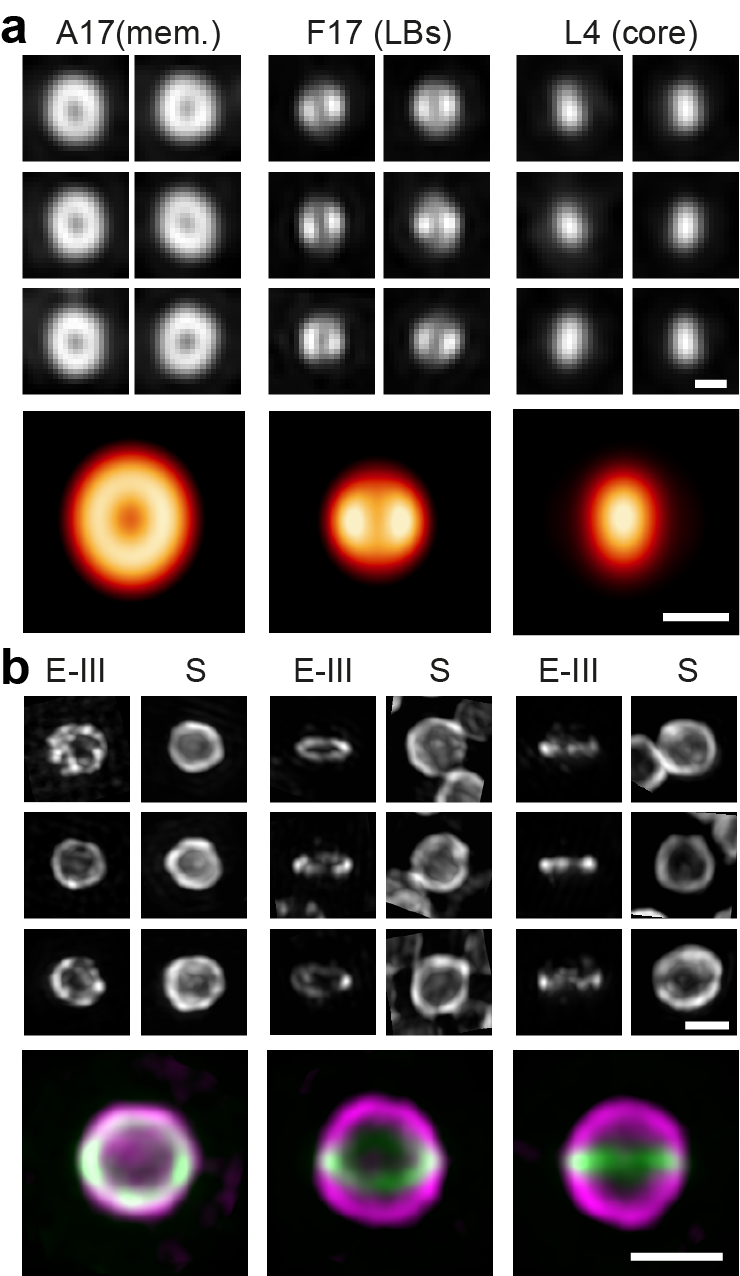
\includegraphics{Figures/FigureVirusMapper_v2.png}
    \caption{\textbf{Quantitative SPA-based modelling with NanoJ-VirusMapper.} \textbf{a)} Top: SIM images of individual vaccinia particles labelled for L4 (core), F17 (lateral body, LB) and A17 (membrane, mem.). Bottom: VirusMapper models of the three channels. Scale bars: 200nm. \textbf{b)} Top: SIM images of individual \emph{Sulfolobus} cells labelled for the S-layer (S) and ESCRT-III (E-III). Bottom: VirusMapper models of three different orientations of the cells. Scale bars: 1\micro m. }
    \label{fig:VirusMapper}
 \end{figure}

\subsection*{NanoJ-Fluidics: Sample Liquid Exchange}

 NanoJ-Fluidics is a hardware and software framework for precise and accurate automated fluidics exchange \cite{almada2018automating}. It was developed to enable automation of sample treatment and labelling of live or fixed cells directly on the microscope stage \cite{dix2018role}. The NanoJ-Fluidics hardware component is composed of customisable, low-cost and robust LEGO® syringe pumps and a fluid removal peristaltic pump, both controlled by simple Arduino® electronics. It is compatible with off-the-shelf imaging chambers, without the need for any microfabrication. Its control software (the NanoJ NanoJ-Fluidics module) is ImageJ-based and can be fully integrated with microscopy acquisition software. We have demonstrated NanoJ-Fluidics' applicability in multiple experimental context: \textit{in-situ} correlative live-to-fixed super-resolution imaging, multimodal super-resolution imaging and event-driven fixation \cite{almada2018automating}, the approach can be easily  extended to protocol optimization (e.g. antibodies concentration or imaging buffer composition) or liquid exchange protocols integrated with the imaging (e.g. drug delivery or automated event-driven fixation).

 Here, we present NanoJ-Fluidics on high-quality multicolour SMLM dataset, by combining STORM and DNA-PAINT \cite{jungmann2014multiplexed} into a single NanoJ-Fluidics workflow (see Fig.\ref{fig:PAINT}a). Our approach is ideally suited to imaging strategies such as multi-label imaging \cite{dempsey2011evaluation}. With NanoJ-Fluidics we can seamlessly perform all labelling steps in an automated and reliable manner directly on the microscope stage. We showcase this with a 4-channel acquisition of actin with STORM and mitochondria, vimentin and clathrin with DNA-PAINT (Fig. \ref{fig:PAINT}b). 

 NanoJ-Fluidics' highly customizable nature has already allowed several alternative designs from the community (\href{https://github.com/HenriquesLab/NanoJ-Fluidics/wiki}{https://github.com/HenriquesLab/NanoJ-Fluidics/wiki}), which are in constant development. NanoJ-Fluidics makes imaging protocol automation available to researchers, this way improving not only the reliability, and repeatability of the protocols but also the scope of protocols that are achievable.  

 %TC:ignore
 \begin{figure}[!t]
    \centering
    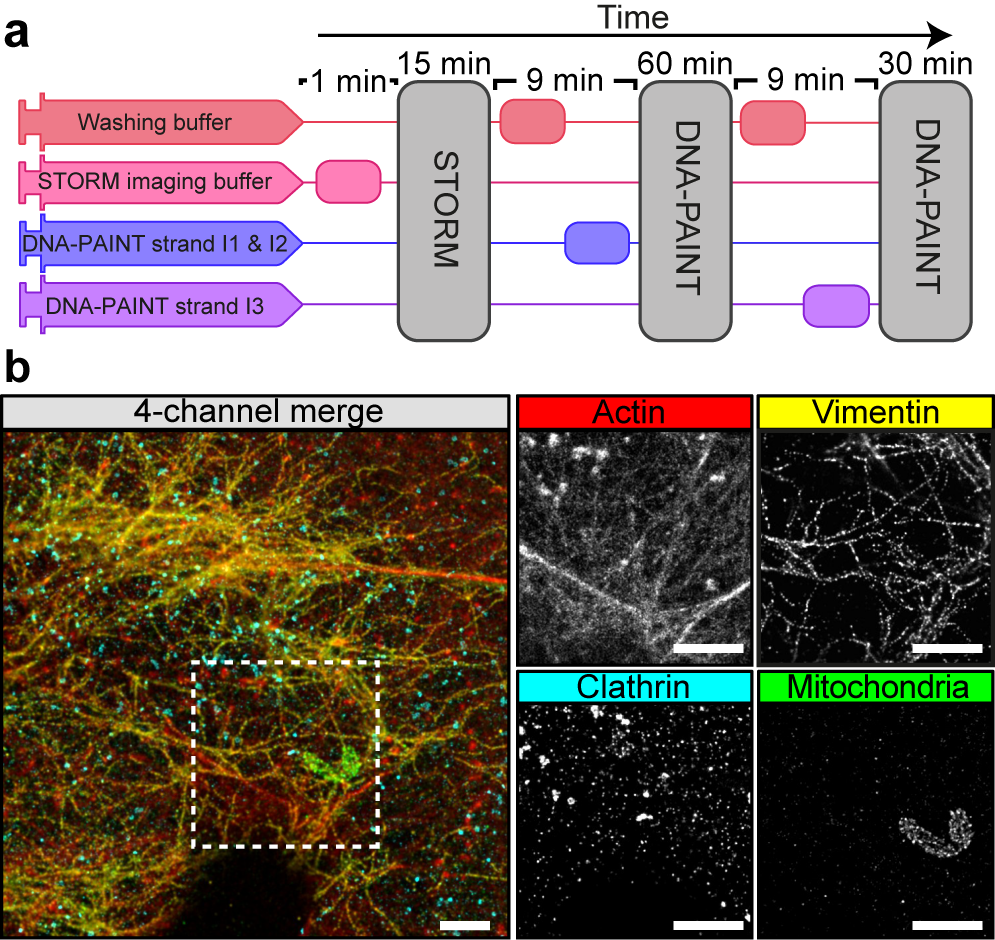
\includegraphics{Figures/FigurePumpy_v3.png}
    \caption{\textbf{Automated DNA-PAINT and STORM imaging.} \textbf{a)} NanoJ-Fluidics workflow used for multi-color STORM and DNA-PAINT imaging. \textbf{b)} 4-channel merge of STORM and DNA-PAINT with actin (red), vimentin (yellow), clathrin (cyan) and mitochondria (green). On the right, Single-channel images from the inset shown on the left. Scale bars: 2 \textmu{}m.}
    \label{fig:PAINT}
 \end{figure}
 %TC:endignore

\subsection*{Discussion and Future Perspectives}
 The NanoJ framework provides a unique and comprehensive set of tools to support cellular imaging along the experimental pathway, from data acquisition and protocol optimisation down to  structural quantification. It offers powerful solutions to common pitfalls of image analysis such as drift correction and channel alignment (NanoJ-Core). Our work on developing analytical approach to SRM (NanoJ-SRRF) aligns with the general aim of the community to extend SRM to live-cell contexts. We also place an emphasis on the importance of quantitatively assessing image data quality not only by a single global resolution metrics but also by spatially-varying FRC resolution maps and error (artefacts) mapping (NanoJ-SQUIRREL). Our work in this context aims at improving standards in assessing and reporting microscopy studies. In our lab, the workflows of live-cell SRRF imaging studies follow the systematic routine of drift/channel alignment and optimisation of acquisition and reconstruction using SQUIRREL. This ensures that our quantitative analysis are of the best scientific standards. NanoJ has been designed for high-performance image analysis, using GPU computing when possible, ensuring the quick processing of large data volumes \cite{herbert2012single,pereira2015high,almada2015palm,beghin2017localization,douglass2016super}. Its modular nature ensures that NanoJ can easily extend the functionality of other SRM software  \cite{sage2018super,weigert2017content,henriques2010quickpalm}. 
 
 We are continuously supporting, adapting and expanding the framework to include new approaches. We hope NanoJ can set a standard of useful, open-source, high performance for the whole microscopy community.
 
\subsection*{Software and Hardware Availability}
 NanoJ follows open-source software and hardware standards. Each of its modules can be installed by enabling the corresponding code repository in Fiji or by following the instructions on the corresponding websites:
 \small
 \begin{itemize}
  \item \href{https://github.com/HenriquesLab/NanoJ-Core}{https://github.com/HenriquesLab/NanoJ-Core}
  \item \href{https://github.com/HenriquesLab/NanoJ-SRRF}{https://github.com/HenriquesLab/NanoJ-SRRF}
  \item \href{https://bitbucket.org/rhenriqueslab/nanoj-squirrel}{https://bitbucket.org/rhenriqueslab/NanoJ-SQUIRREL}
  \item \href{https://bitbucket.org/rhenriqueslab/NanoJ-VirusMapper}{https://bitbucket.org/rhenriqueslab/NanoJ-VirusMapper}
  \item \href{https://github.com/HenriquesLab/NanoJ-Fluidics}{https://github.com/HenriquesLab/NanoJ-Fluidics}
\end{itemize}

\begin{acknowledgements}
 We thank Prof. Ralf Jungmann at Max Planck Institute of Biochemistry Munich for reagents and advice. This work was funded by grants from the UK Biotechnology and Biological Sciences Research Council (BB/M022374/1; BB/P027431/1; BB/R000697/1; BB/S507532/1) (R.H., P.M.P. and R.F.L.), the UK Medical Research Council (MR/K015826/1) (R.H.), the Wellcome Trust (203276/Z/16/Z) (S.C., R.H and B.B.) and the Centre National de la Recherche Scientifique (CNRS ATIP-AVENIR program AO2016) (C.L.). N.G. and R.D.M.G funded by the Engineering and Physical Sciences Research Council (EP/L504889/1). P.A. was supported by a PhD fellowship from the UK’s Biotechnology and Biological Sciences Research Council. Research by B.B. was supported by UCL, Cancer Research UK (C1529/A17343), and MRC (MC\_CF12266). K.L.T. and G.T.R. supported by a 4-year MRC Research Studentship.
\end{acknowledgements}

\begin{contributions}
 These contributions follow the Contributor Roles Taxonomy guidelines: \href{https://casrai.org/credit/}{https://casrai.org/credit/}.
 Conceptualization: K.L.T, R.F.L., N.G., R.D.M.G, P.A., D.A., G.T.R., B.B., J.M., C.L., P.M.P., S.C., R.H.;
 Data curation: K.L.T, R.F.L., R.D.M.G, G.T.R., J.M., C.L., P.M.P., S.C., R.H.;
 Formal analysis:  K.L.T, R.F.L., R.D.M.G, C.L., S.C.;
 Funding acquisition:  B.B., C.L., R.H.;
 Investigation: K.L.T, R.F.L., R.D.M.G, G.T.R., C.L., P.M.P., S.C.;
 Methodology: R.F.L., N.G., R.D.M.G, P.A., J.M., C.L., P.M.P., S.C., R.H.;
 Project administration: R.F.L., B.B., J.M., C.L., P.M.P., S.C., R.H.;
 Resources: K.L.T, R.D.M.G, D.A., G.T.R., A.L., B.B., J.M., C.L., P.M.P., S.C.;
 Software: R.F.L., N.G., R.D.M.G, P.A., C.L., P.M.P., S.C., R.H.;
 Supervision: R.F.L., A.L., B.B., J.M., C.L., P.M.P., S.C., R.H.;
 Validation: K.L.T, R.F.L., N.G., R.D.M.G, P.A., D.A., C.L., P.M.P., S.C.;
 Visualization:  K.L.T, R.F.L., R.D.M.G, D.A., C.L., P.M.P., S.C., R.H.;
 Writing – original draft: K.L.T, R.F.L., R.D.M.G, D.A., C.L., P.M.P., S.C., R.H.;
 Writing – review \& editing: all authors.

\end{contributions}

\begin{interests}
 The authors declare no competing financial interests.
\end{interests}

\section*{Bibliography}
\bibliographystyle{zHenriquesLab-StyleBib}
\bibliography{06_Bibliography_Clean}
